\chapter{Intersection unit modeling}
\label{appendix:app_intersection_modeling}

\section{Cycle-accurate simulation of mean cycles-per-intersection, compared between several intersection units}

\begin{table}
\centering
\caption{Average Cycles Per Intersection}
\begin{tabular}{|c|c|c|c|c|c|c|}
\toprule
 fibLen &  vecLen &  s0 &  s1 &  Direct-mapped &  Naive radix-2 &  Skip-ahead radix-2 \\
\midrule
      4 &       1 & 0.2 & 0.5 &            1.0 &          1.000 &               1.357 \\
      4 &       1 & 0.2 & 0.8 &            1.0 &          1.000 &               1.606 \\
      4 &       1 & 0.5 & 0.8 &            1.0 &          1.000 &               1.497 \\
      4 &       2 & 0.2 & 0.5 &            1.0 &          2.225 &               1.769 \\
      4 &       2 & 0.2 & 0.8 &            1.0 &          1.655 &               1.642 \\
      4 &       2 & 0.5 & 0.8 &            1.0 &          1.580 &               1.700 \\
      4 &       4 & 0.2 & 0.5 &            1.0 &          3.370 &               3.110 \\
      4 &       4 & 0.2 & 0.8 &            1.0 &          2.540 &               2.140 \\
      4 &       4 & 0.5 & 0.8 &            1.0 &          1.630 &               1.850 \\
     32 &       1 & 0.2 & 0.5 &            1.0 &          1.000 &               1.439 \\
     32 &       1 & 0.2 & 0.8 &            1.0 &          1.000 &               1.720 \\
     32 &       1 & 0.5 & 0.8 &            1.0 &          1.000 &               1.614 \\
     32 &       2 & 0.2 & 0.5 &            1.0 &          2.225 &               1.870 \\
     32 &       2 & 0.2 & 0.8 &            1.0 &          2.272 &               1.933 \\
     32 &       2 & 0.5 & 0.8 &            1.0 &          2.248 &               2.027 \\
     32 &       4 & 0.2 & 0.5 &            1.0 &          4.593 &               3.041 \\
     32 &       4 & 0.2 & 0.8 &            1.0 &          4.754 &               2.670 \\
     32 &       4 & 0.5 & 0.8 &            1.0 &          4.930 &               3.080 \\
    256 &       1 & 0.2 & 0.5 &            1.0 &          1.000 &               1.442 \\
    256 &       1 & 0.2 & 0.8 &            1.0 &          1.000 &               1.756 \\
    256 &       1 & 0.5 & 0.8 &            1.0 &          1.000 &               1.658 \\
    256 &       2 & 0.2 & 0.5 &            1.0 &          2.228 &               1.876 \\
    256 &       2 & 0.2 & 0.8 &            1.0 &          2.374 &               1.943 \\
    256 &       2 & 0.5 & 0.8 &            1.0 &          2.385 &               2.037 \\
    256 &       4 & 0.2 & 0.5 &            1.0 &          4.620 &               3.019 \\
    256 &       4 & 0.2 & 0.8 &            1.0 &          5.057 &               2.651 \\
    256 &       4 & 0.5 & 0.8 &            1.0 &          5.115 &               2.945 \\
\bottomrule
\end{tabular}
\end{table}

\newpage

\begin{figure}[H]
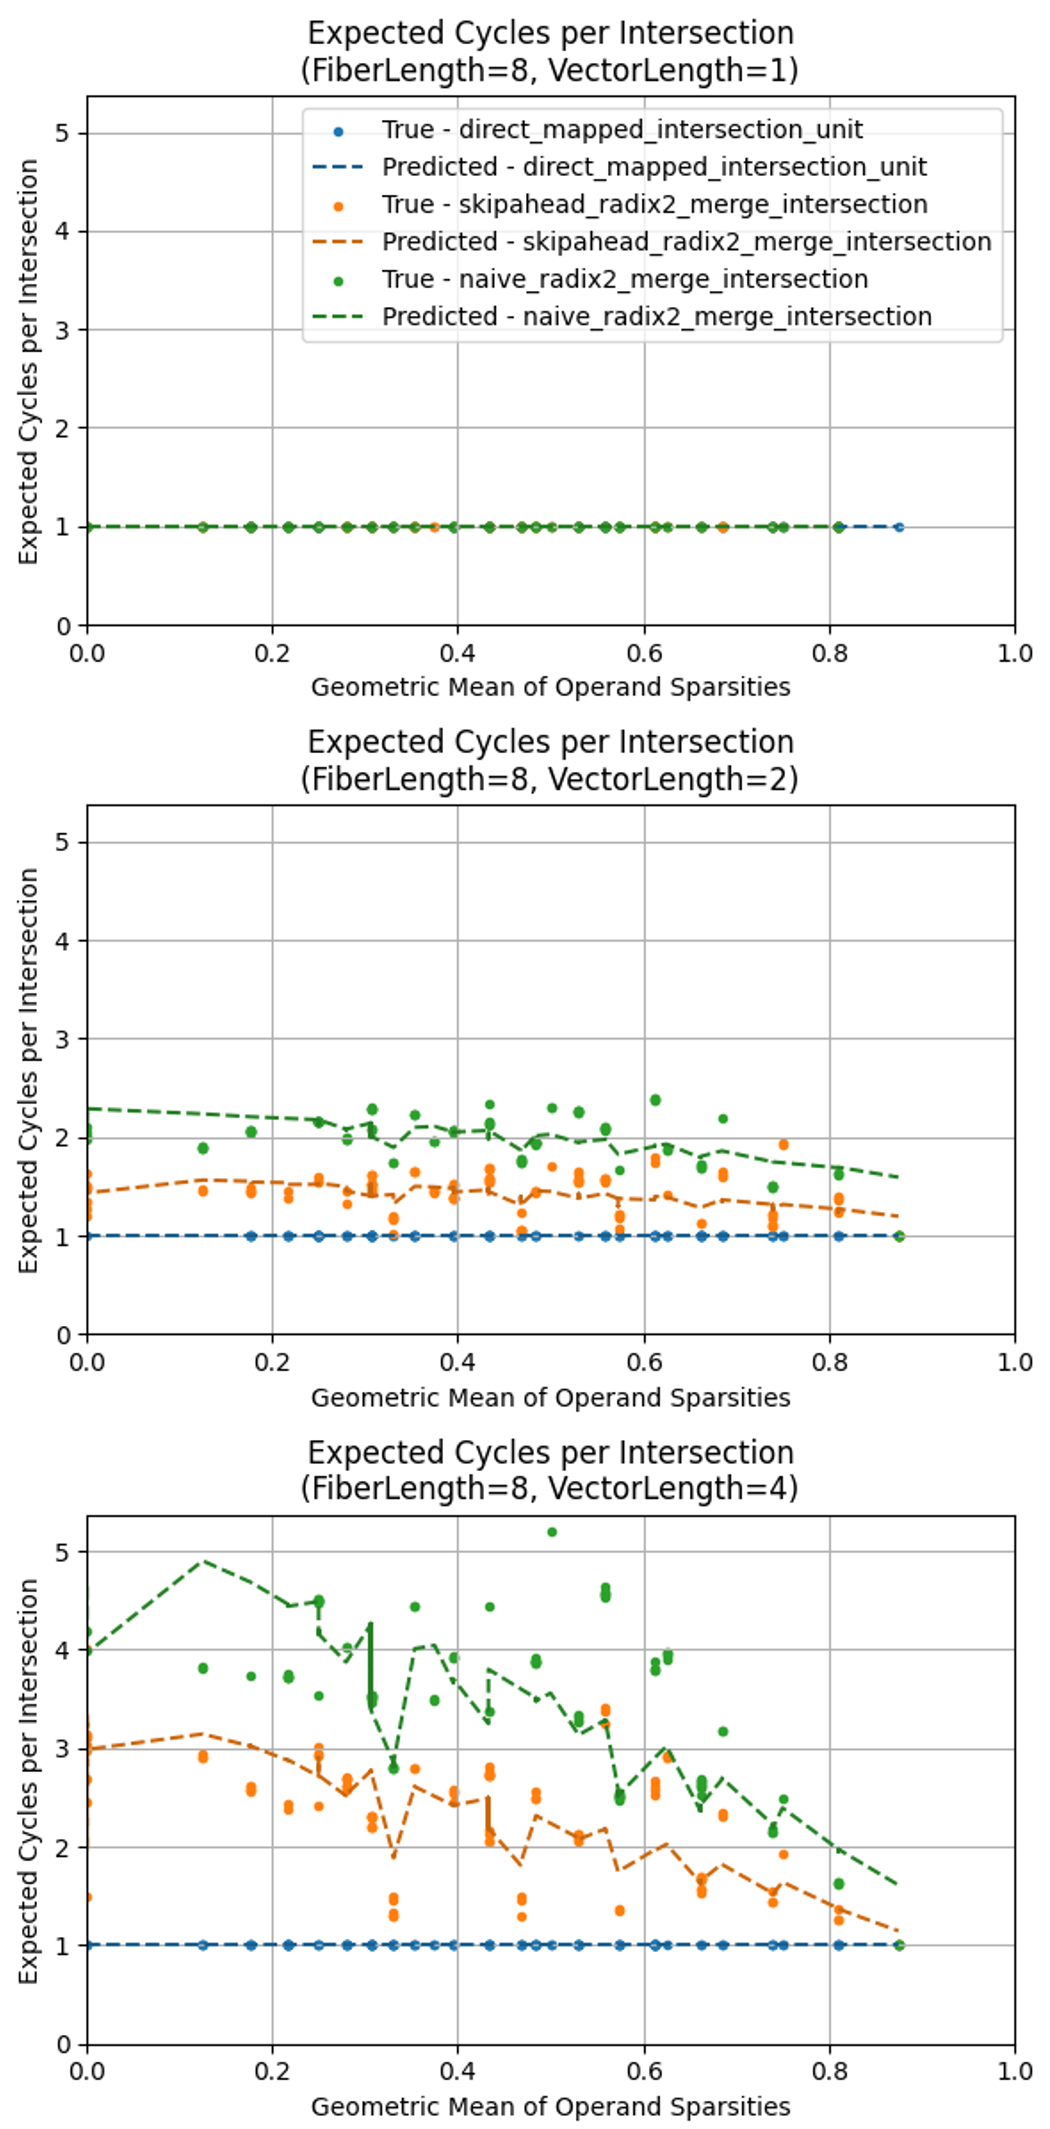
\includegraphics[width=0.75\textwidth]{figures/expected_cycles_F8.png}
\caption{Average cycles-per-intersection when applying a $\{1,2,4\}$-way vectorized intersection unit to intersect two length-8 vectors. Naive two-fingered merge, skip-ahead, and direct-mapped intersection units are compared.}
\label{fig:expected_cycles_F8}
\end{figure}

\newpage

\begin{figure}[H]
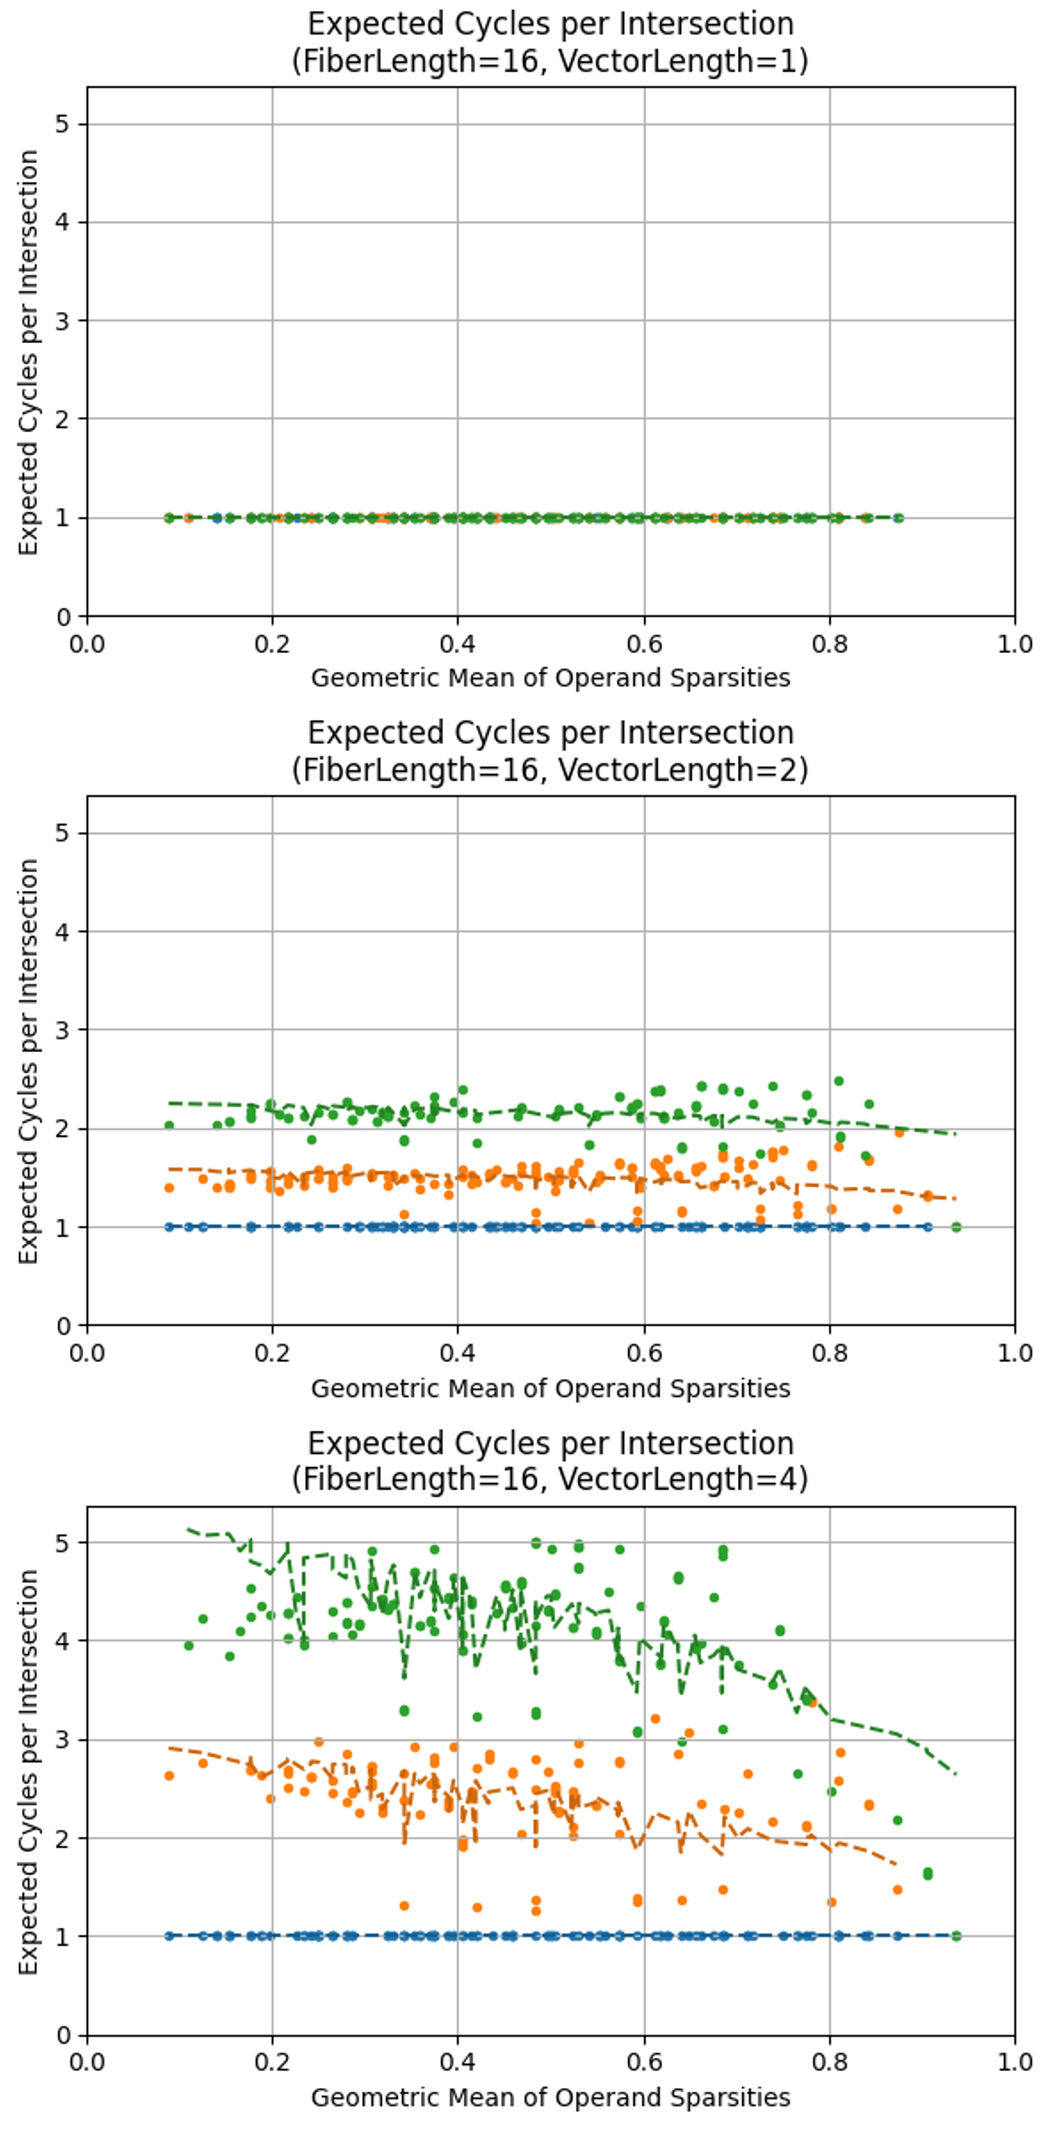
\includegraphics[width=0.75\textwidth]{figures/expected_cycles_F16.png}
\caption{Average cycles-per-intersection when applying a $\{1,2,4\}$-way vectorized intersection unit to intersect two length-16 vectors. Naive two-fingered merge, skip-ahead, and direct-mapped intersection units are compared.}
\label{fig:expected_cycles_F16}
\end{figure}

\newpage

\begin{figure}[H]
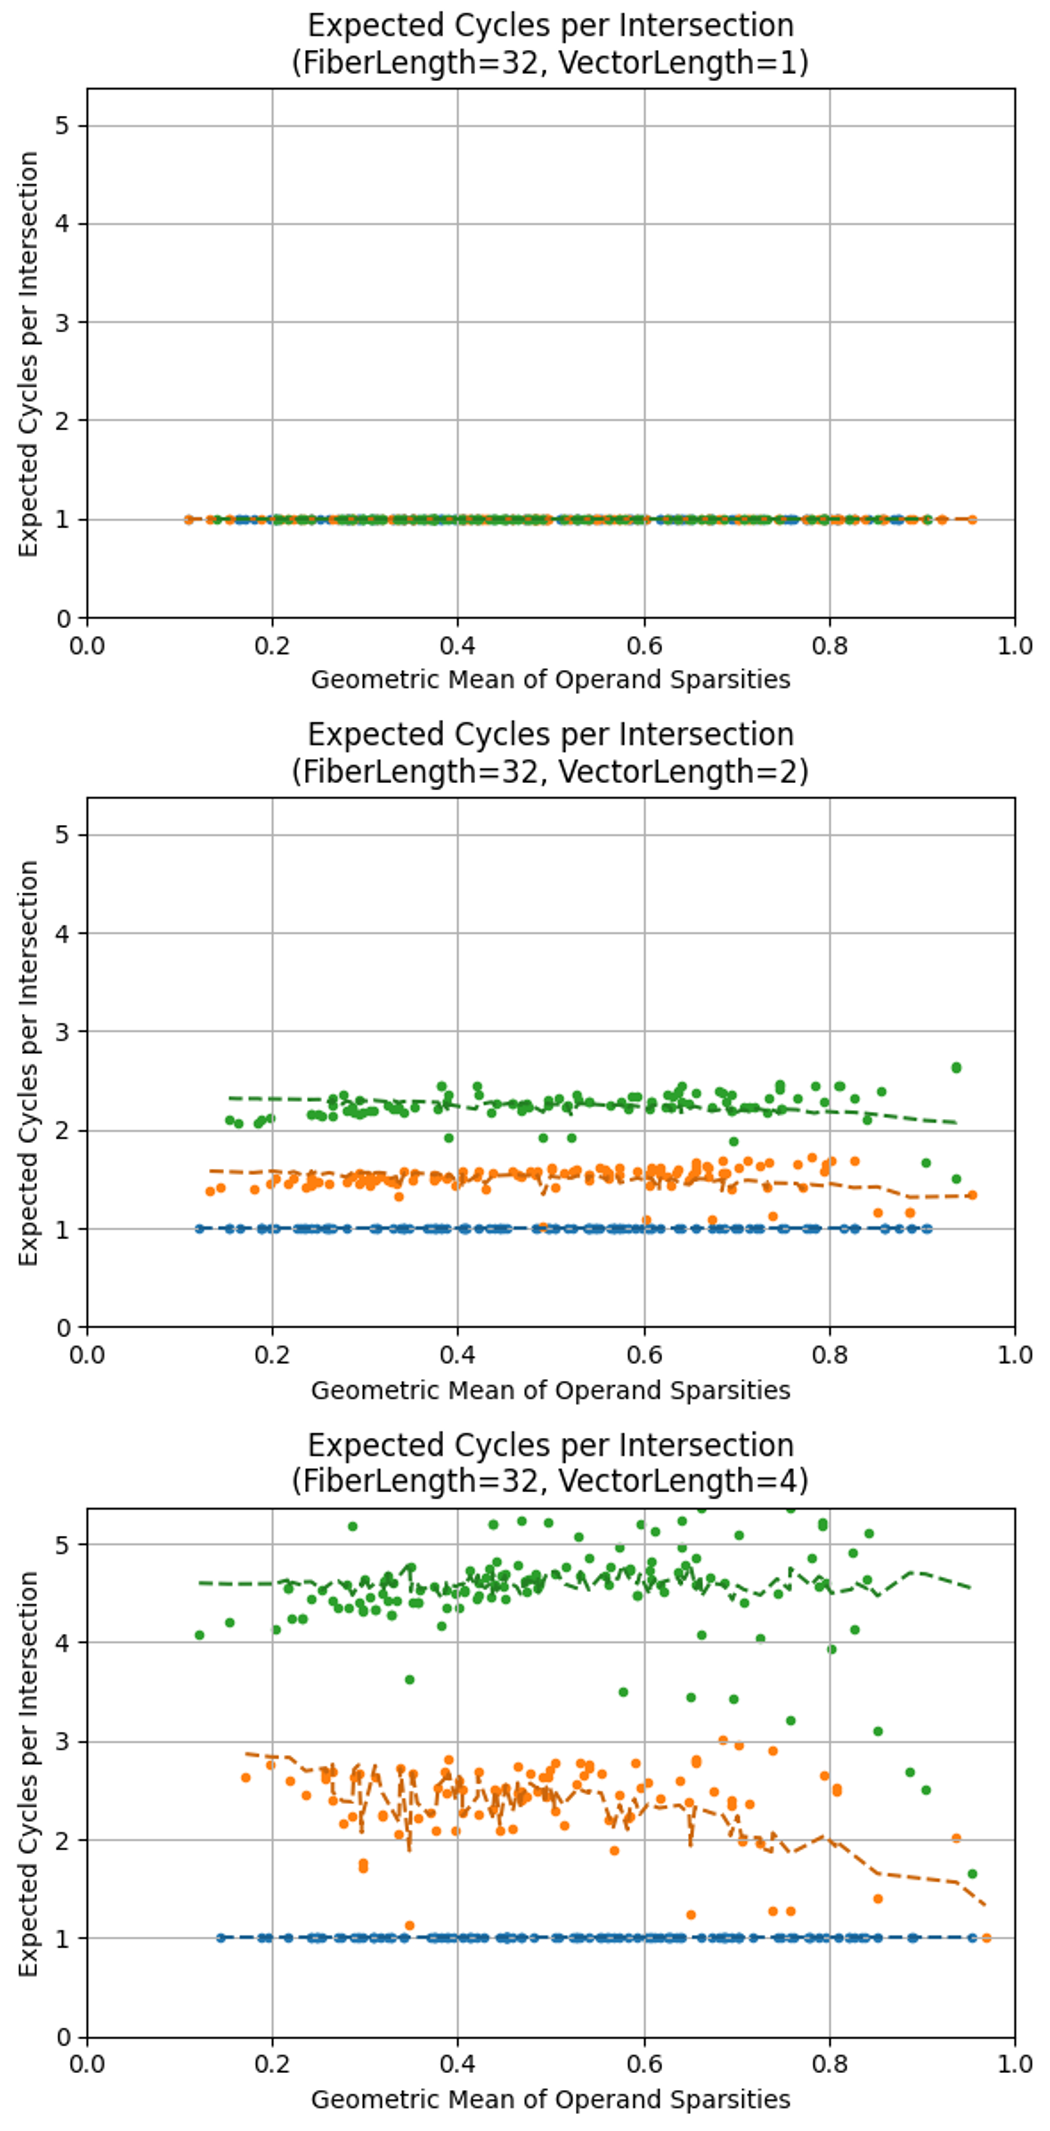
\includegraphics[width=0.75\textwidth]{figures/expected_cycles_F32.png}
\caption{Average cycles-per-intersection when applying a $\{1,2,4\}$-way vectorized intersection unit to intersect two length-32 vectors. Naive two-fingered merge, skip-ahead, and direct-mapped intersection units are compared.}
\label{fig:expected_cycles_F32}
\end{figure}

\clearpage

\section{Detailed comparison of match throughput as a function of sparsity (geomean) for several varieties of intersection unit, several fiber size values, and several unique degrees of input vectorization.}

\begin{figure}[H]
    \centering
    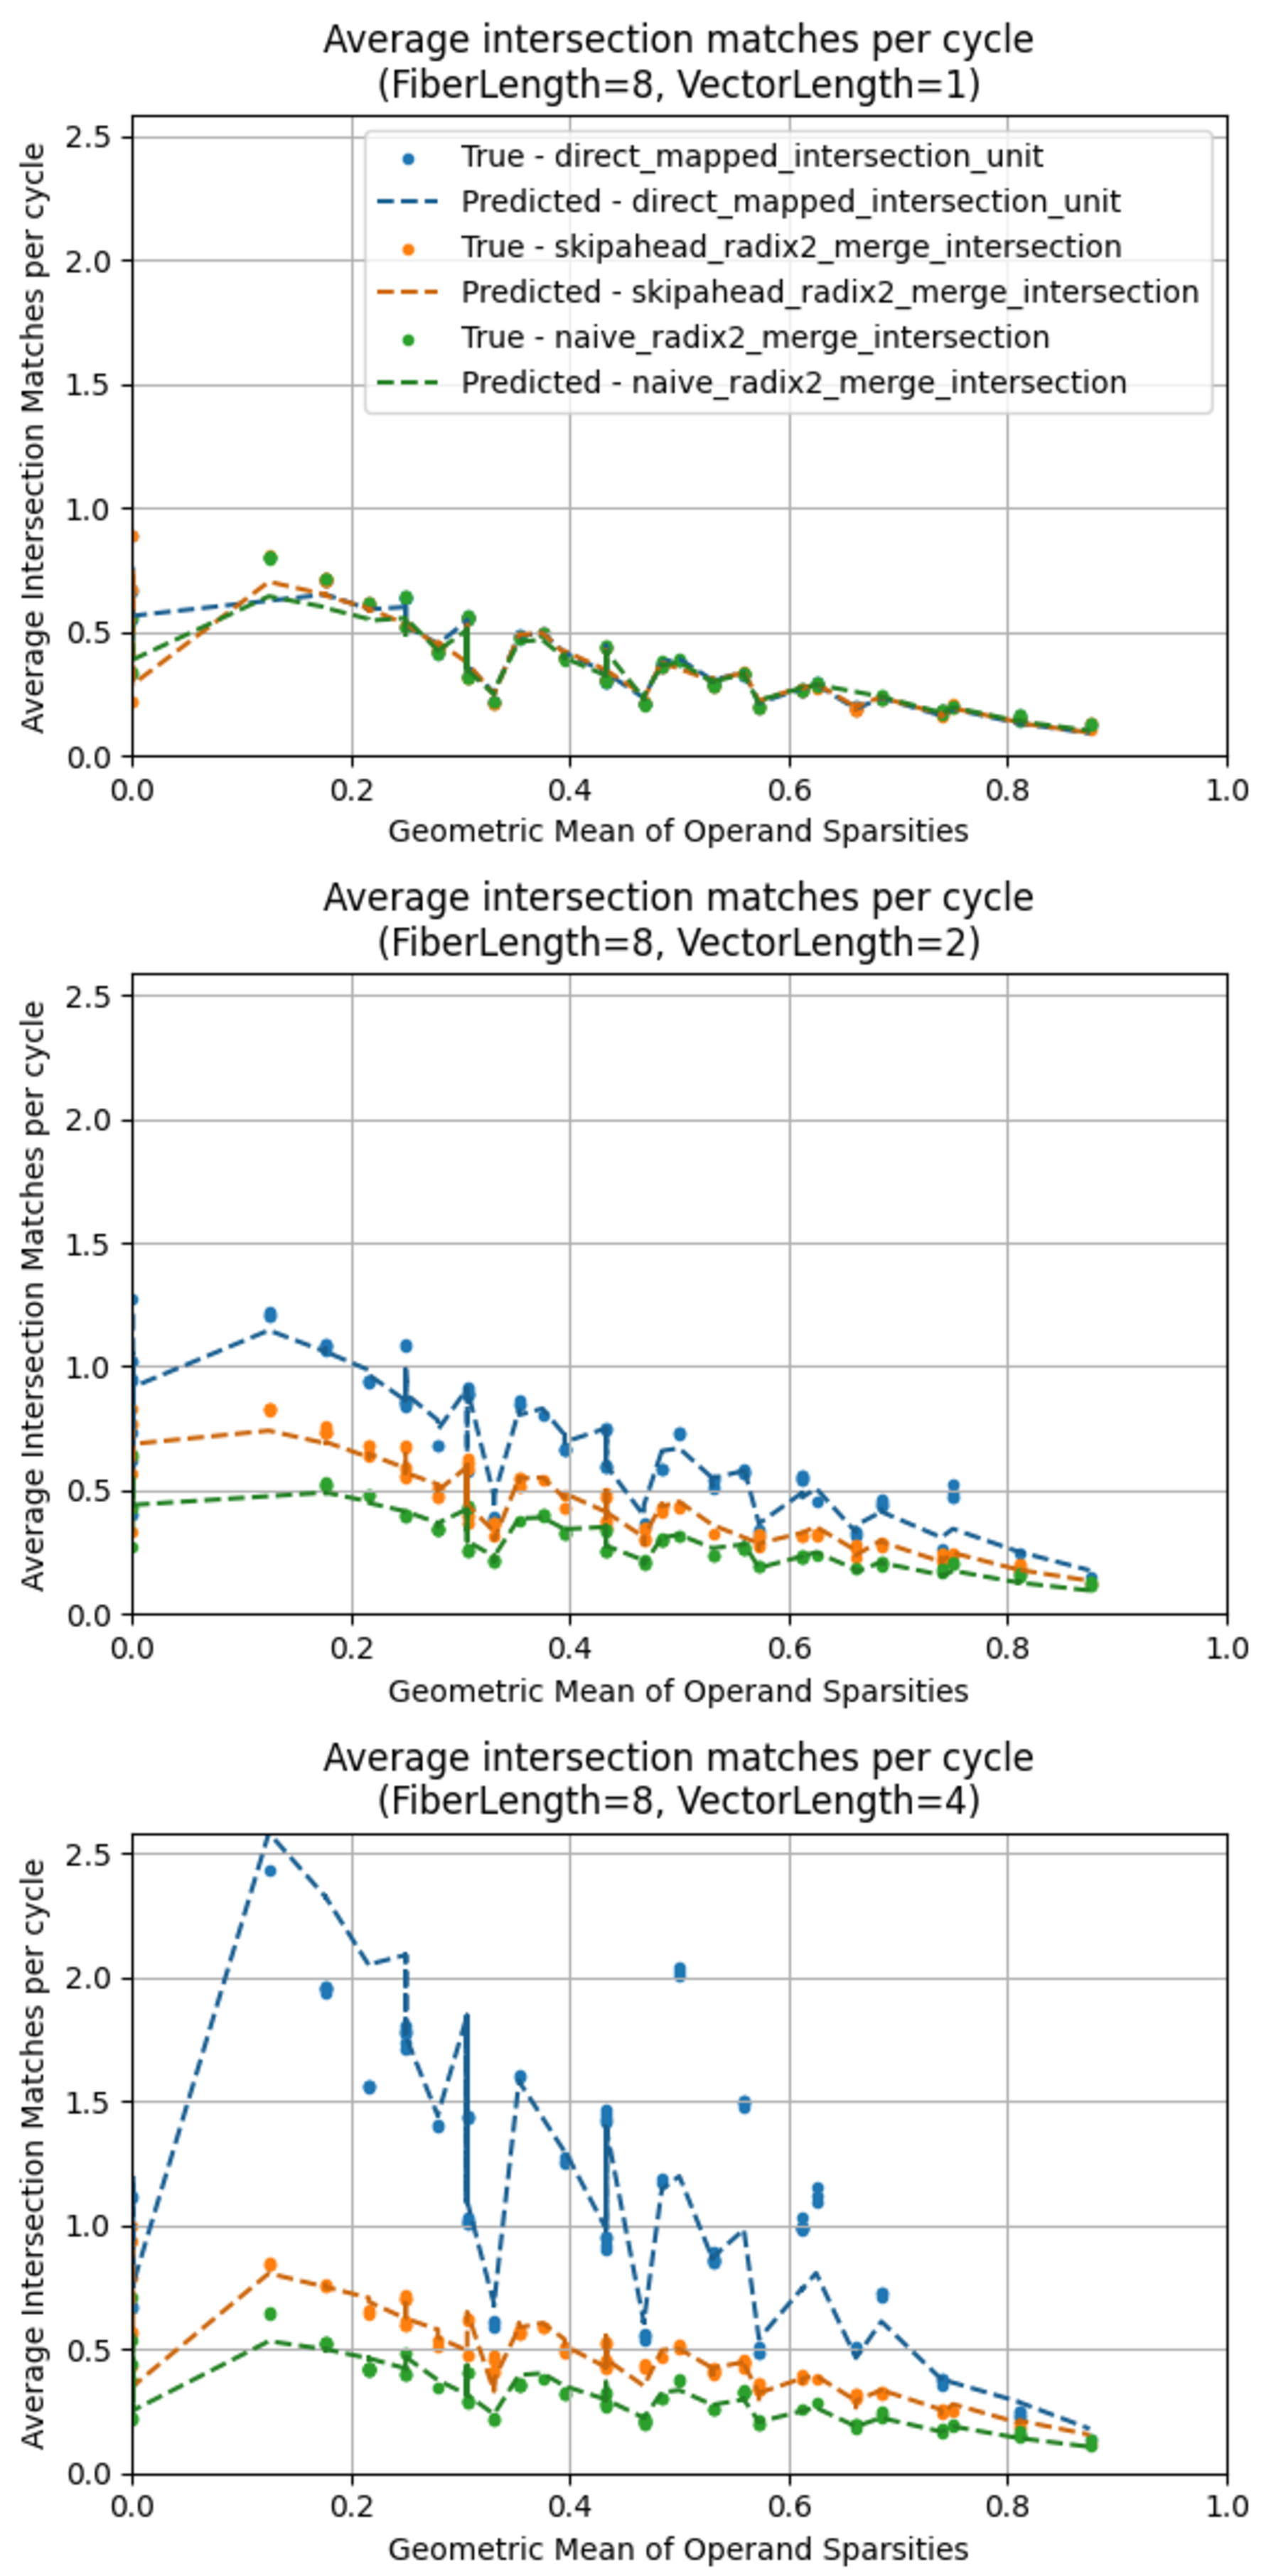
\includegraphics[width=0.8\textwidth]{figures/isect_model_fl8_vl1.pdf}
    \caption{Comparison of match throughput with respect to sparsity (geomean) for fiber size 8 and input vectorization degrees 1, 2 and 4.}
    \label{fig:isect_model_fl8_vl1}
\end{figure}

\clearpage

\begin{figure}[H]
    \centering
    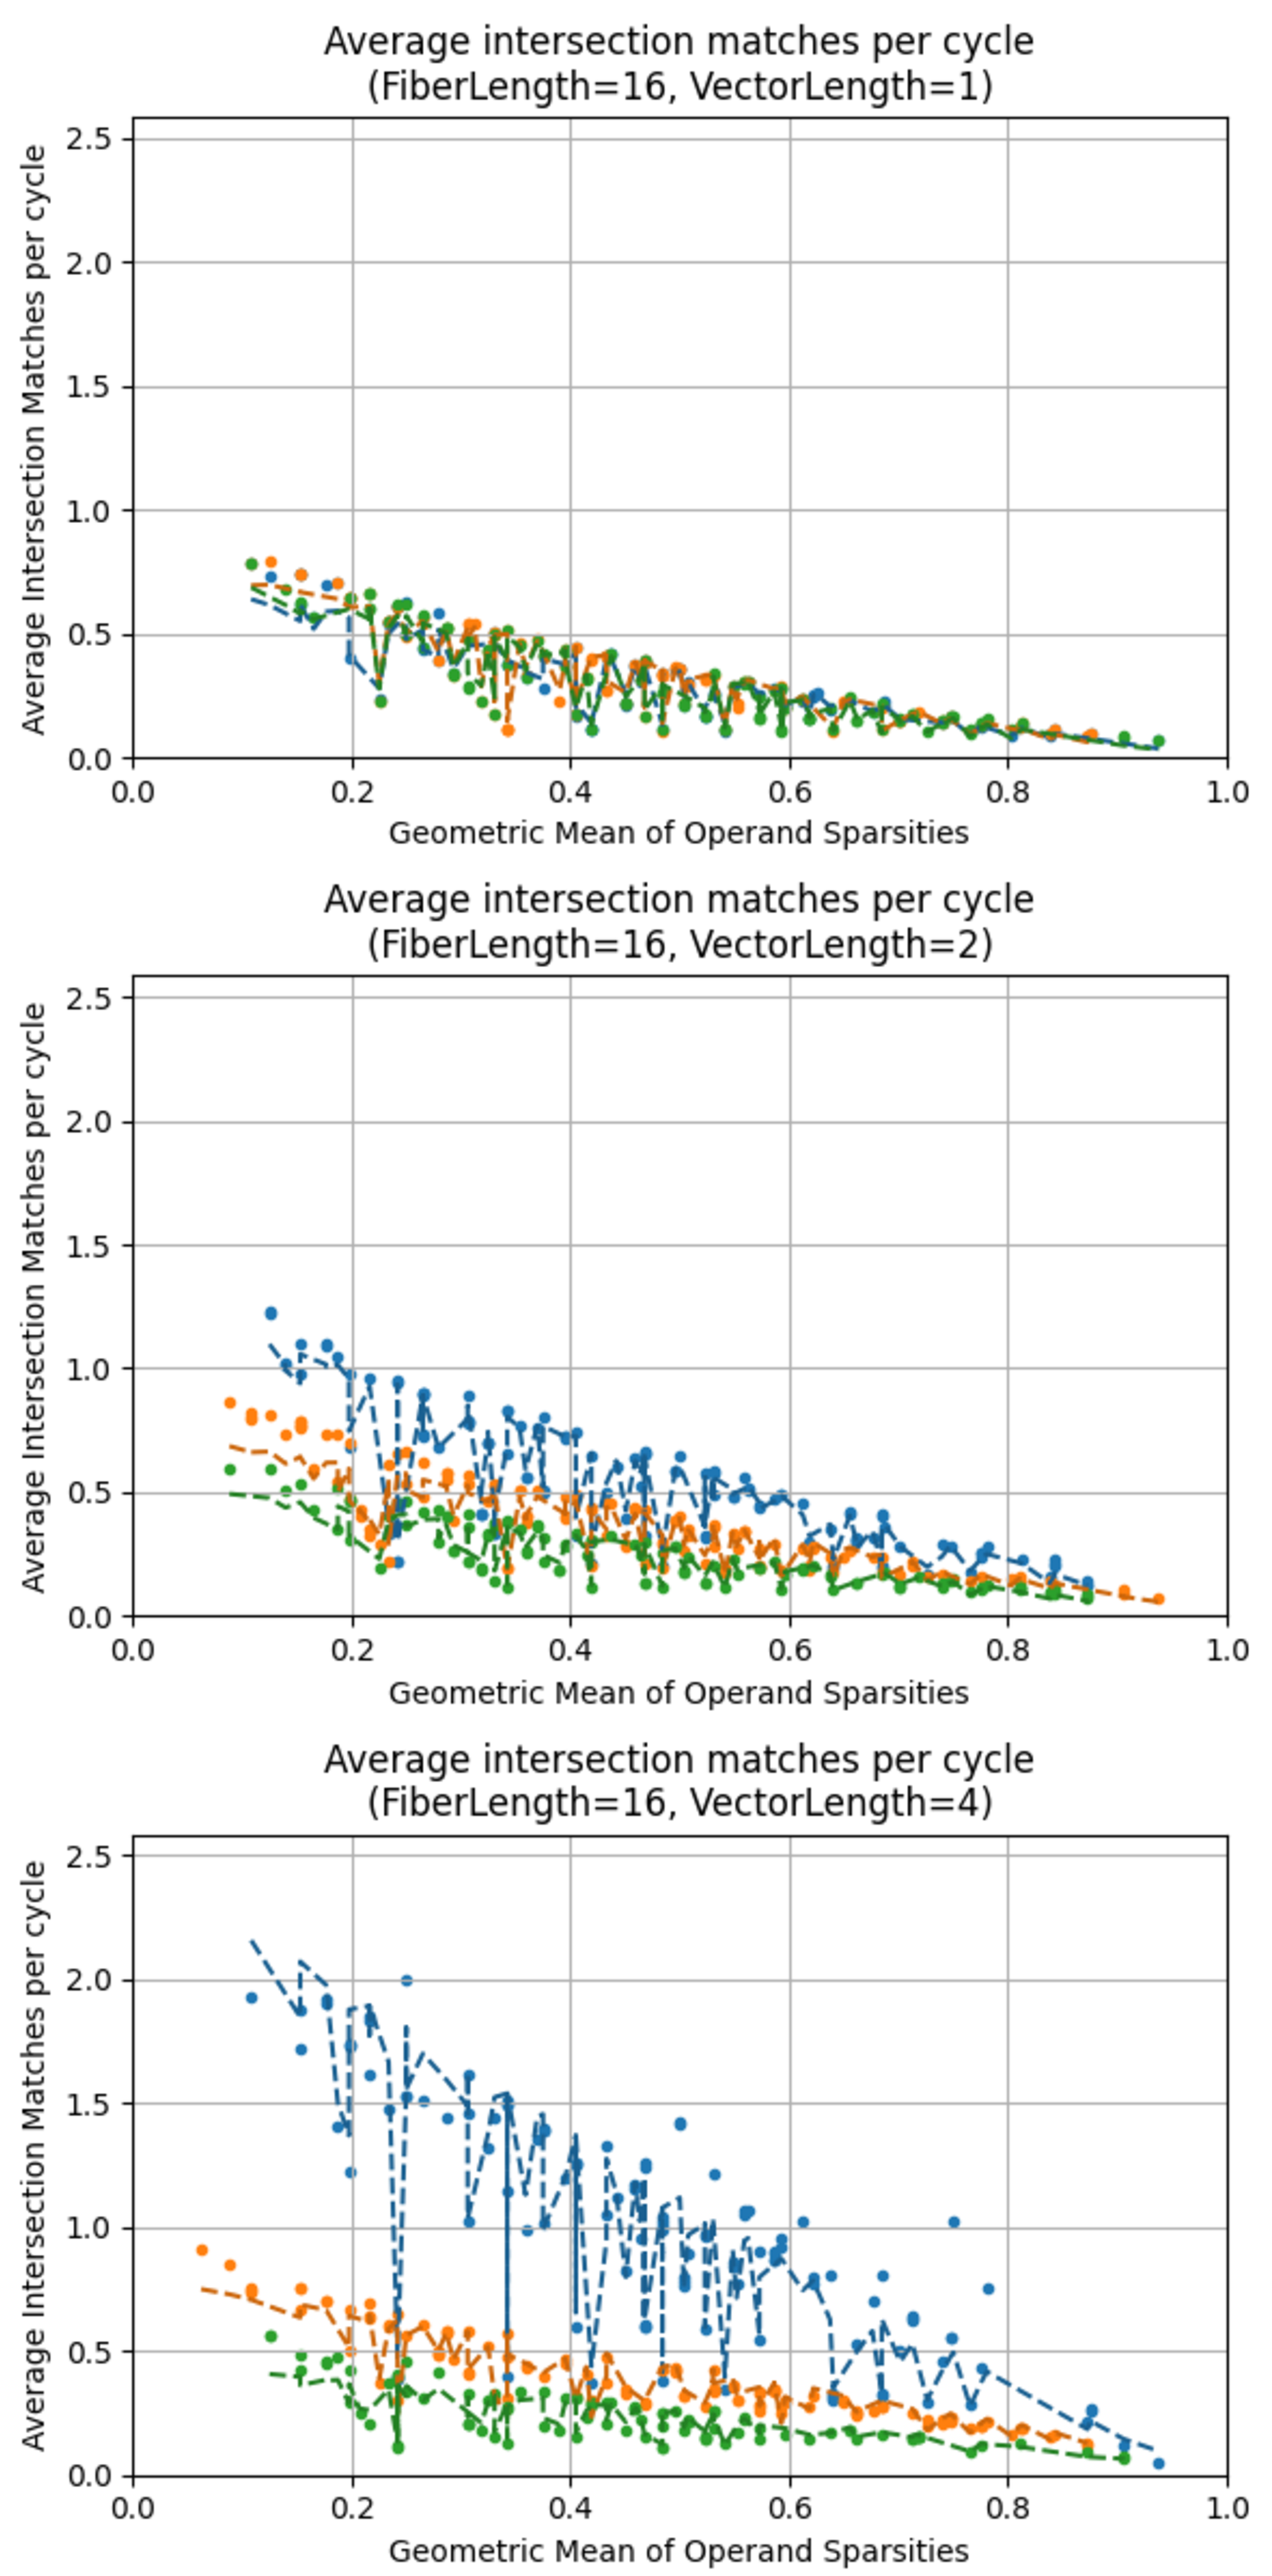
\includegraphics[width=0.8\textwidth]{figures/isect_model_fl16_vl1.pdf}
    \caption{Comparison of match throughput with respect to sparsity (geomean) for fiber size 16 and vectorization degrees 1, 2 and 4.}
    \label{fig:isect_model_fl16_vl1}
\end{figure}

\clearpage

\begin{figure}[H]
    \centering
    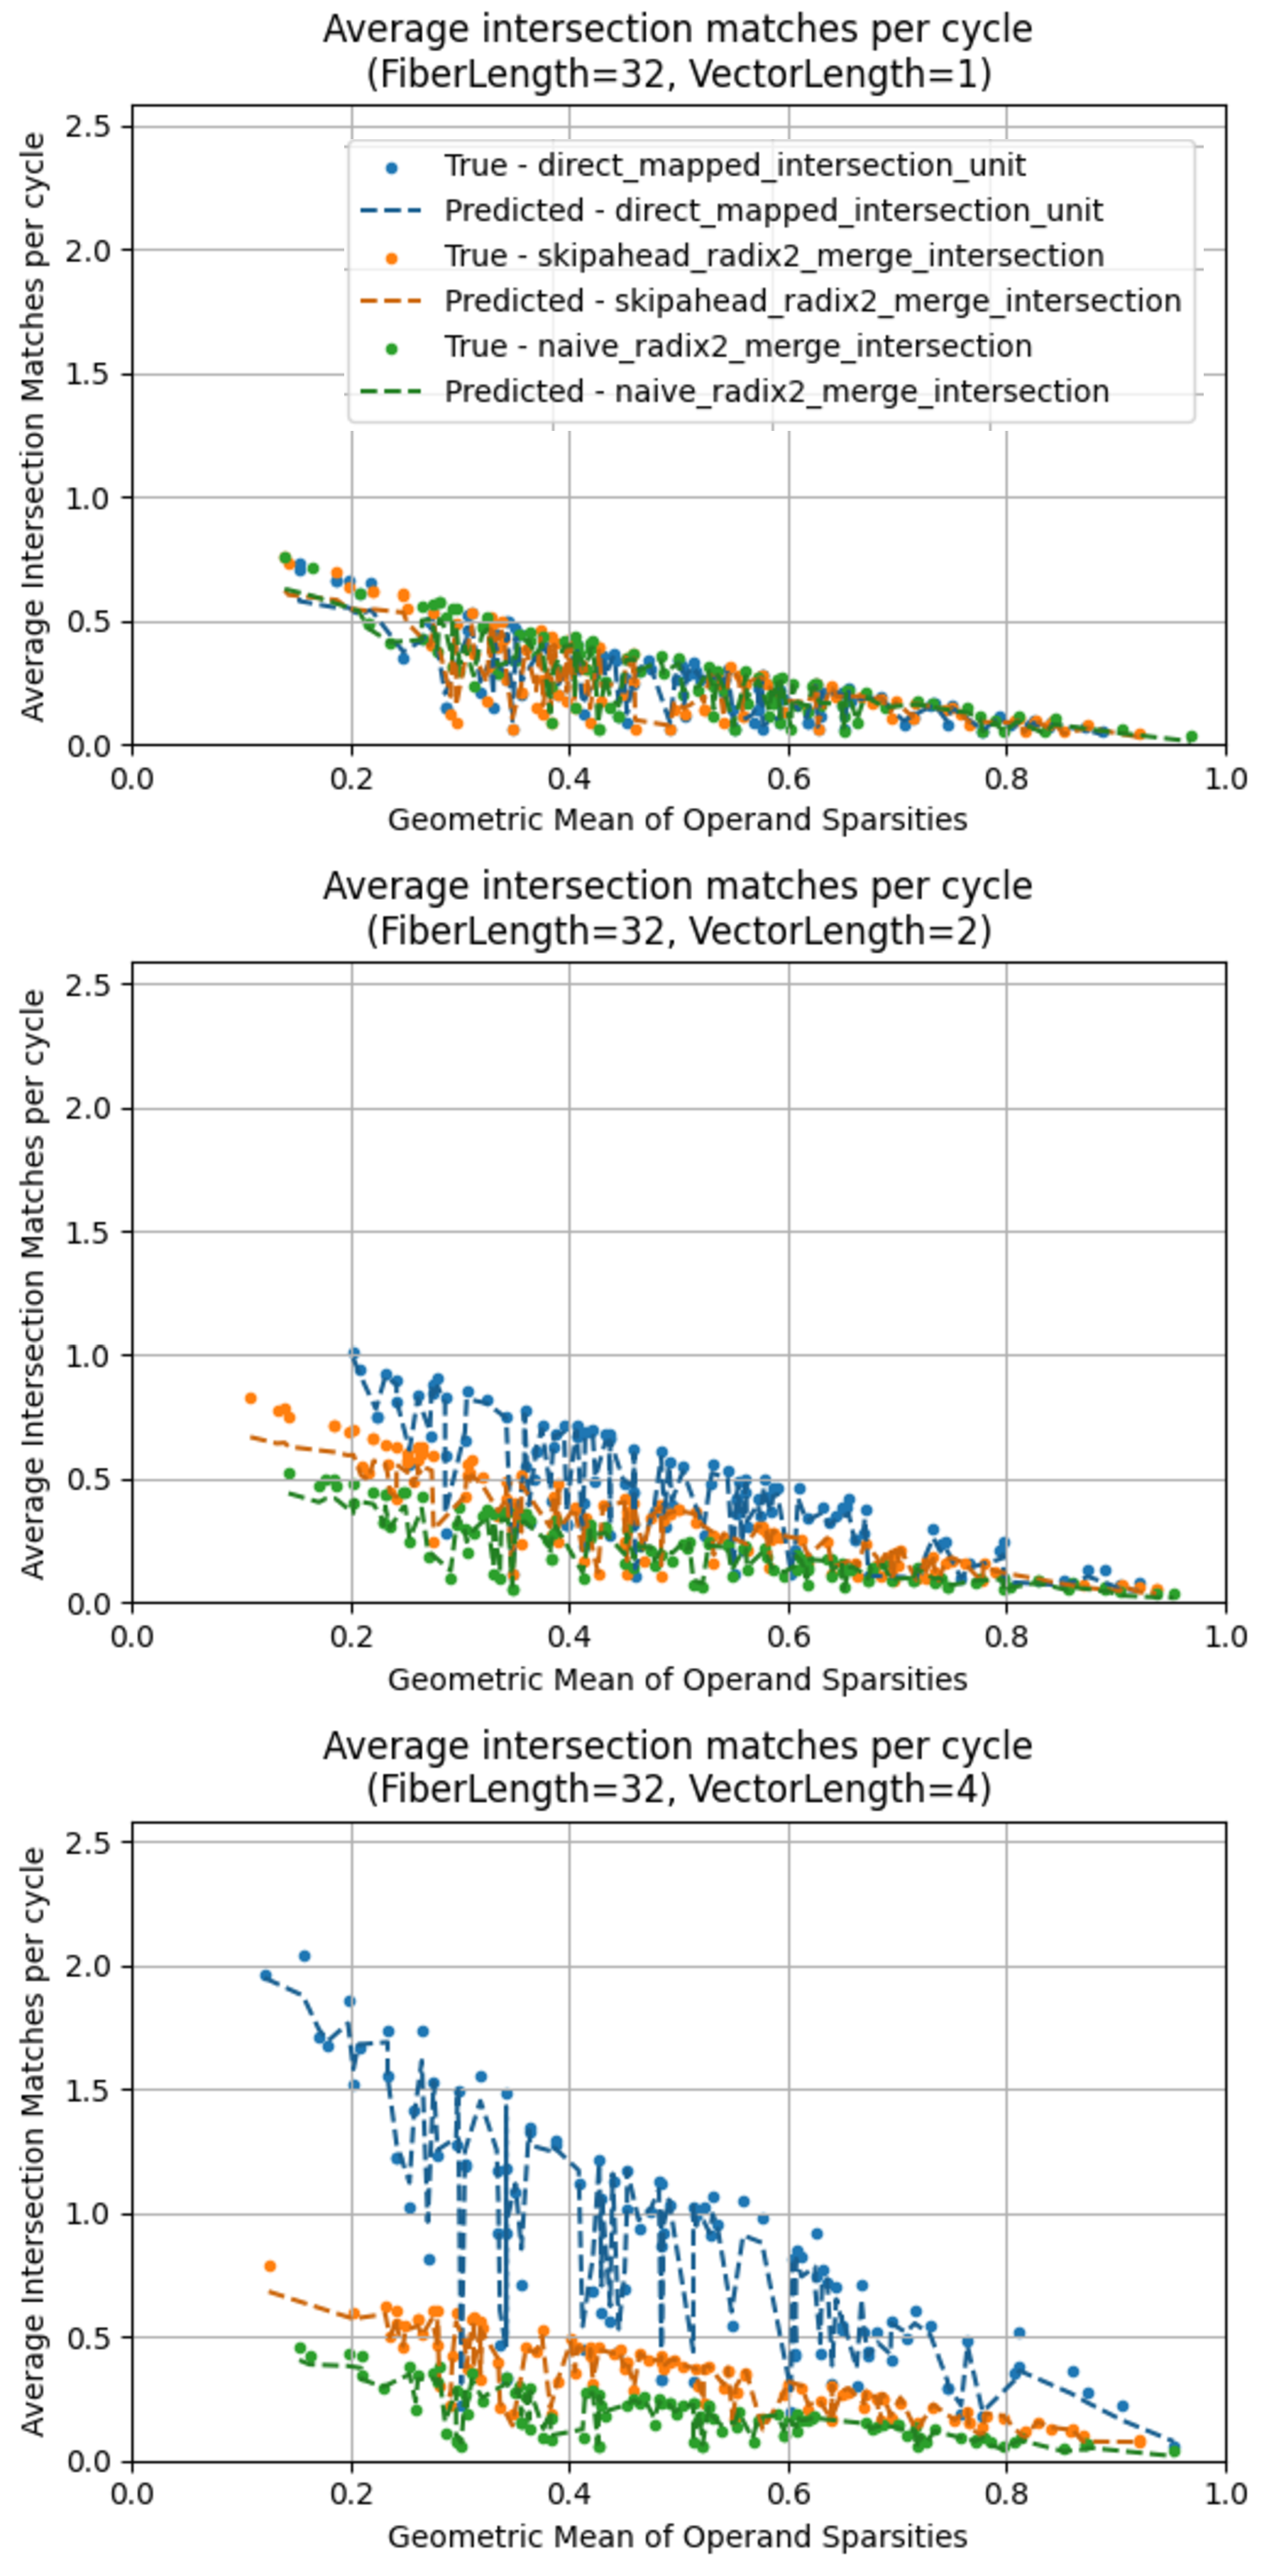
\includegraphics[width=0.8\textwidth]{figures/isect_model_fl32_vl1.pdf}
    \caption{Comparison of match throughput with respect to sparsity (geomean) for fiber size 32 and input vectorization degrees 1, 2 and 4.}
    \label{fig:isect_model_fl32_vl1}
\end{figure}

\clearpage